%% Requires compilation with XeLaTeX or LuaLaTeX
\documentclass[aspectratio=169,10pt,xcolor={table,dvipsnames},t]{beamer}
\usetheme{UCBerkeley}
\hypersetup{colorlinks=true, linkcolor=blue, citecolor=blue, urlcolor=blue}
\usepackage{xcolor}

\title[lecture 09]{Next Generation Data Centers and Energy Management Systems}
\subtitle{Lecture 9A: Machine Learning and Optimization Tools}
\author{Prof. Thomas M. Schutzius}
\institute{Department of Mechanical Engineering}
\date{Fall 2026}

\begin{document}

\begin{frame}
  \titlepage
\end{frame}

% Uncomment these lines for an automatically generated outline.
%\begin{frame}{Outline}
%  \tableofcontents
%\end{frame}

{
\smallframetitle % small frame title
\setbeamertemplate{background}{} % Hides background for this frame
\setbeamertemplate{footline}{}   % Reclaims the bottom space

% Learning plan. Highlight in bold the item we are covering in this lecture.
\begin{frame}
	\frametitle{Learning Plan}
	\begin{itemize}
		\item Introduction to Data Center Systems and Thermodynamics 
		\item Psychrometrics and Heat Transfer
		\item Performance Metrics and Standards
		\item Applied Computational Fluid Dynamics (CFD)
		\item Liquid Cooling \& Advanced Heat Transfer
		\item Chip Cooling: Heat Conduction and Thermal Interface Materials
		\item Power Delivery and Infrastructure (Energy sources: Geothermal, Solar, Nuclear, etc.)
		\item Overview of Simulation Field; the Concept of a Digital Twin
		\item \textbf{Machine Learning and Optimization Tools}
		\item Modeling and Simulation of an Energy Management System 
		\item Control Systems and Optimization 
		\item Spacecraft Thermal Control
		\item Final Project Work, Peer Feedback, and Mentor Check-in 
		\item Symposium 
	\end{itemize}		
\end{frame}

% Learning objectives go here.
\begin{frame}
	\frametitle{Learning Objectives} 
		\begin{itemize}
			\item Develop the principles of classical optimization methods
			\item Develop and apply a modern optimization technique (genetic algorithm) to optimizing rack layout in a data center
%			\item ...%Create a reduced order model for a 2D transient heat conduction problem with heat generation
%			\item Modeling 2D transient heat conduction in heterogeneous materials.
		\end{itemize}		
\end{frame}


% Include the typical layout of a data center facility in each lecture.
\begin{frame}
	\frametitle{Typical layout of a data center facility}
		\begin{figure}
			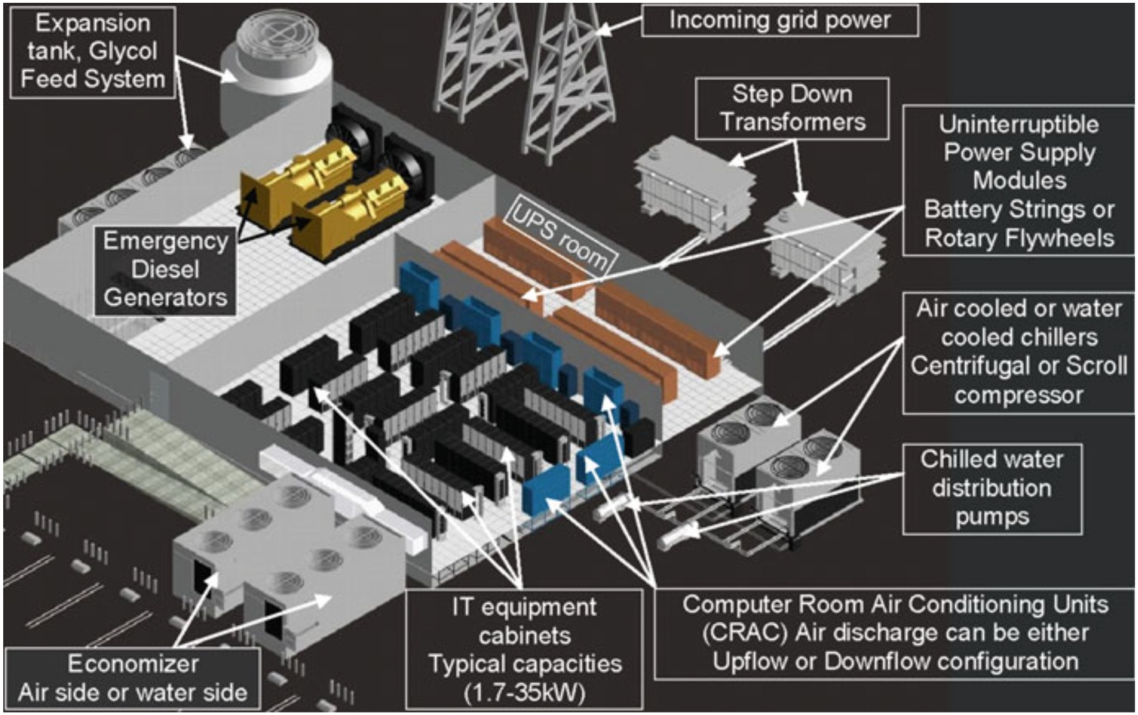
\includegraphics[width=0.65\textwidth]{../figures/joshi2021introduction-figure-01-01.pdf}
%			\vspace{-0.5cm }
		 \caption{(Figure 1.1 in Ref. \cite{joshi2012energy}).}
		\end{figure}
\end{frame}


\begin{frame}
	\frametitle{Seminar 6}
		\begin{itemize}
			\item Surya Swamy and Aniket Soneji, Hammerhead AI
			\item Title: Turning Stranded Power into AI Inference-ready Capacity
			\item Date: October 30, 2026
			\item Time: 10:00 (Berkeley Time)
			\item Location: EH 3110 (Seminar Room)
		\end{itemize}
\end{frame}

\begin{frame}
	\frametitle{Seminar 7}
		\begin{itemize}
			\item Sherman Ikemoto, Cadence
			\item Title: Dynamic Infrastructure: Digital Twin Architecture for Next-Generation AI Factories
			\item Date: November 5, 2026
			\item Time: 15:30 (Berkeley Time)
			\item Location: GSPP 150
		\end{itemize}
\end{frame}

\begin{frame}
	\frametitle{Seminar 8}
		\begin{itemize}
			\item Alex Lotz, AWS
			\item Title: TBD
			\item Date: November 5, 2026
			\item Time: 15:30 (Berkeley Time)
			\item Location: GSPP 150
		\end{itemize}
\end{frame}

    \begin{frame}
        \frametitle{\href{https://datahub.berkeley.edu/user-redirect/git-pull?repo=https://github.com/mtsn-lab/me137-237a&subPath=examples/optimizationMethodsIntroduction.ipynb}{Optimization}}

%            \begin{figure}
%                \centering
%                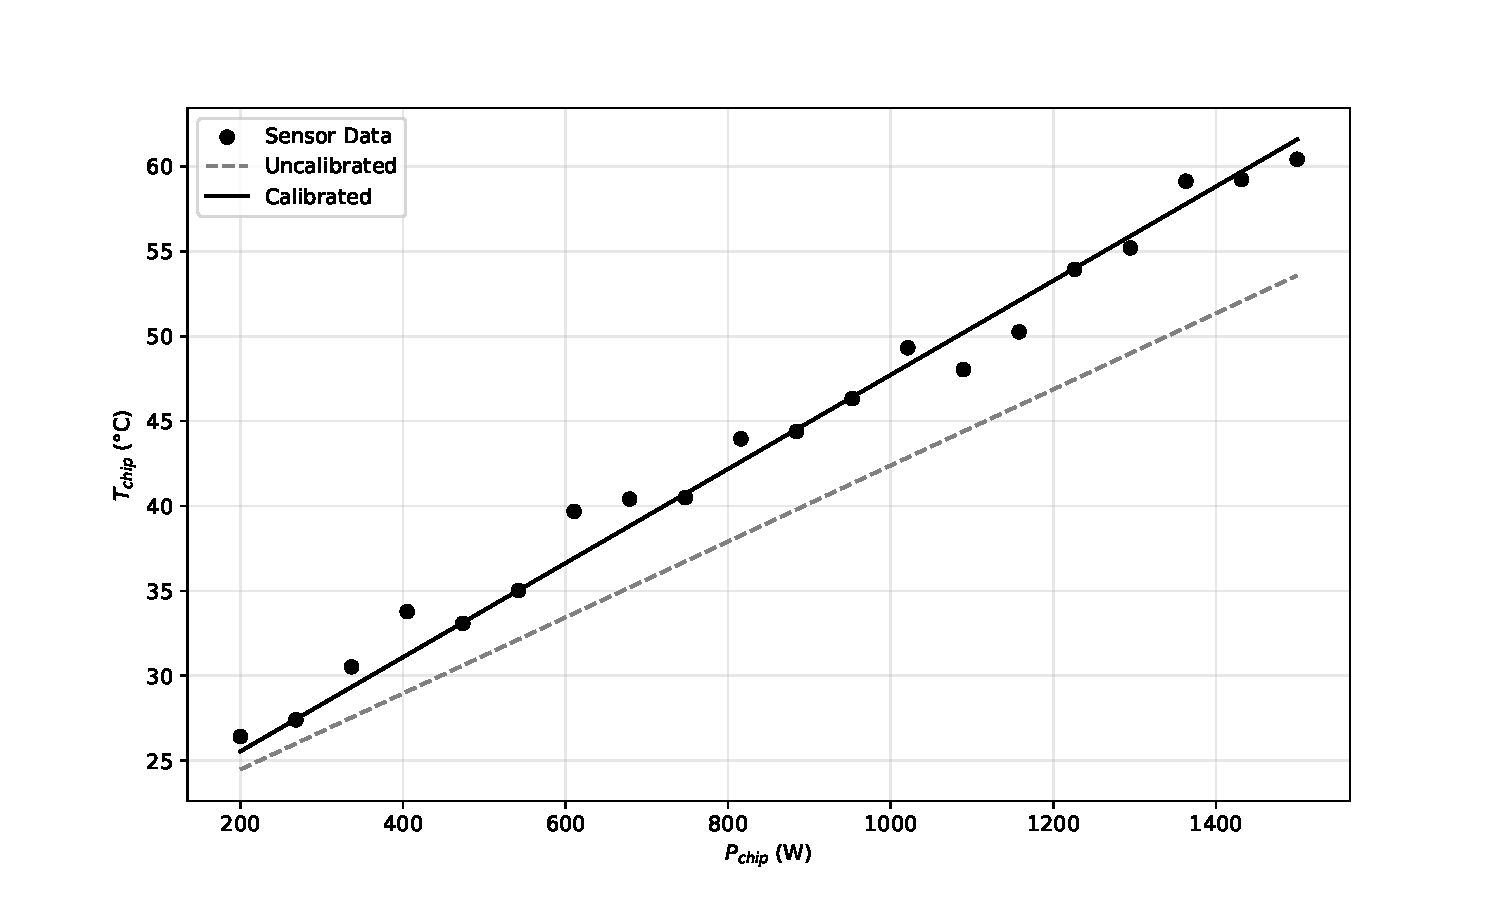
\includegraphics[width=0.7\textwidth]{../figures/digital_twin_chip_temperature.pdf}
%                 \caption{Calibrating a digital twin.}
%            \end{figure}
    \end{frame}


    \begin{frame}
        \frametitle{\href{https://datahub.berkeley.edu/user-redirect/git-pull?repo=https://github.com/mtsn-lab/me137-237a&subPath=examples/optimizationGeneticAlgorithmRackLayout.ipynb}{Optimizing the layout of racks in a data center hall}}

%            \begin{figure}
%                \centering
%                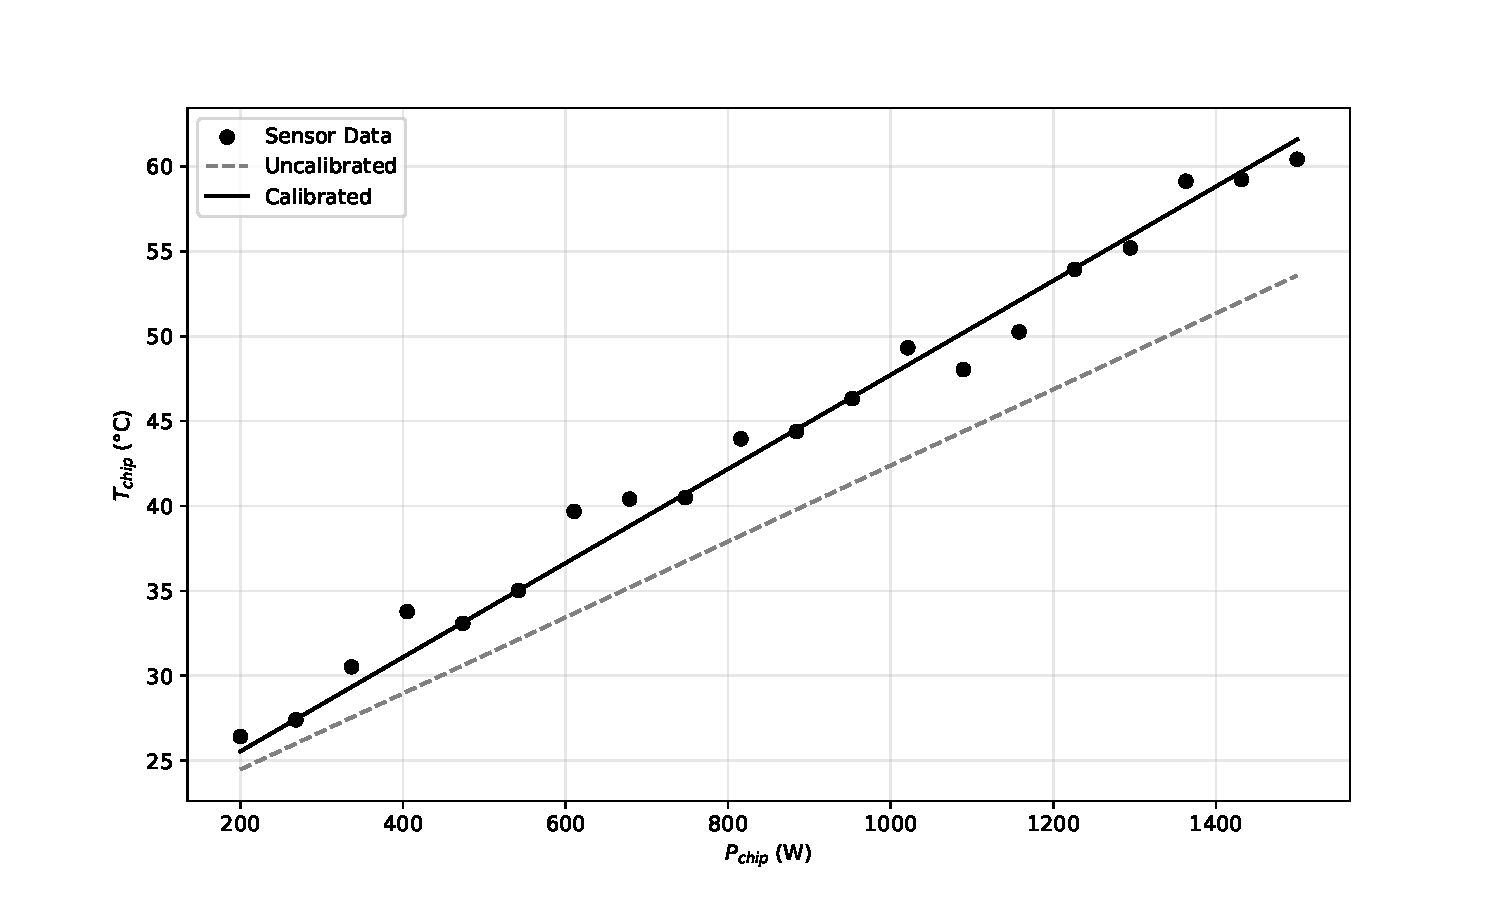
\includegraphics[width=0.7\textwidth]{../figures/digital_twin_chip_temperature.pdf}
%                 \caption{Calibrating a digital twin.}
%            \end{figure}
    \end{frame}

    

% ------------------------------------------------------------------------------------------------------------------------------------------------------------------------------------
% This is an example for how I link the Jupyter notebook example to the slide I am showing.
% If there is a figure output from the Jupyter notebook, that should be shown here. The Jupyter notebook should be located in me137-237a/examples
% The figure output from the Jupyter notebook should go in the directory me137-237a/lectures/figures

%\begin{frame}
%	\frametitle{\href{https://datahub.berkeley.edu/user-redirect/git-pull?repo=https://github.com/mtsn-lab/me137-237a&subPath=examples/fanLaws.ipynb}{Fan Laws}}
%		\begin{figure}
%			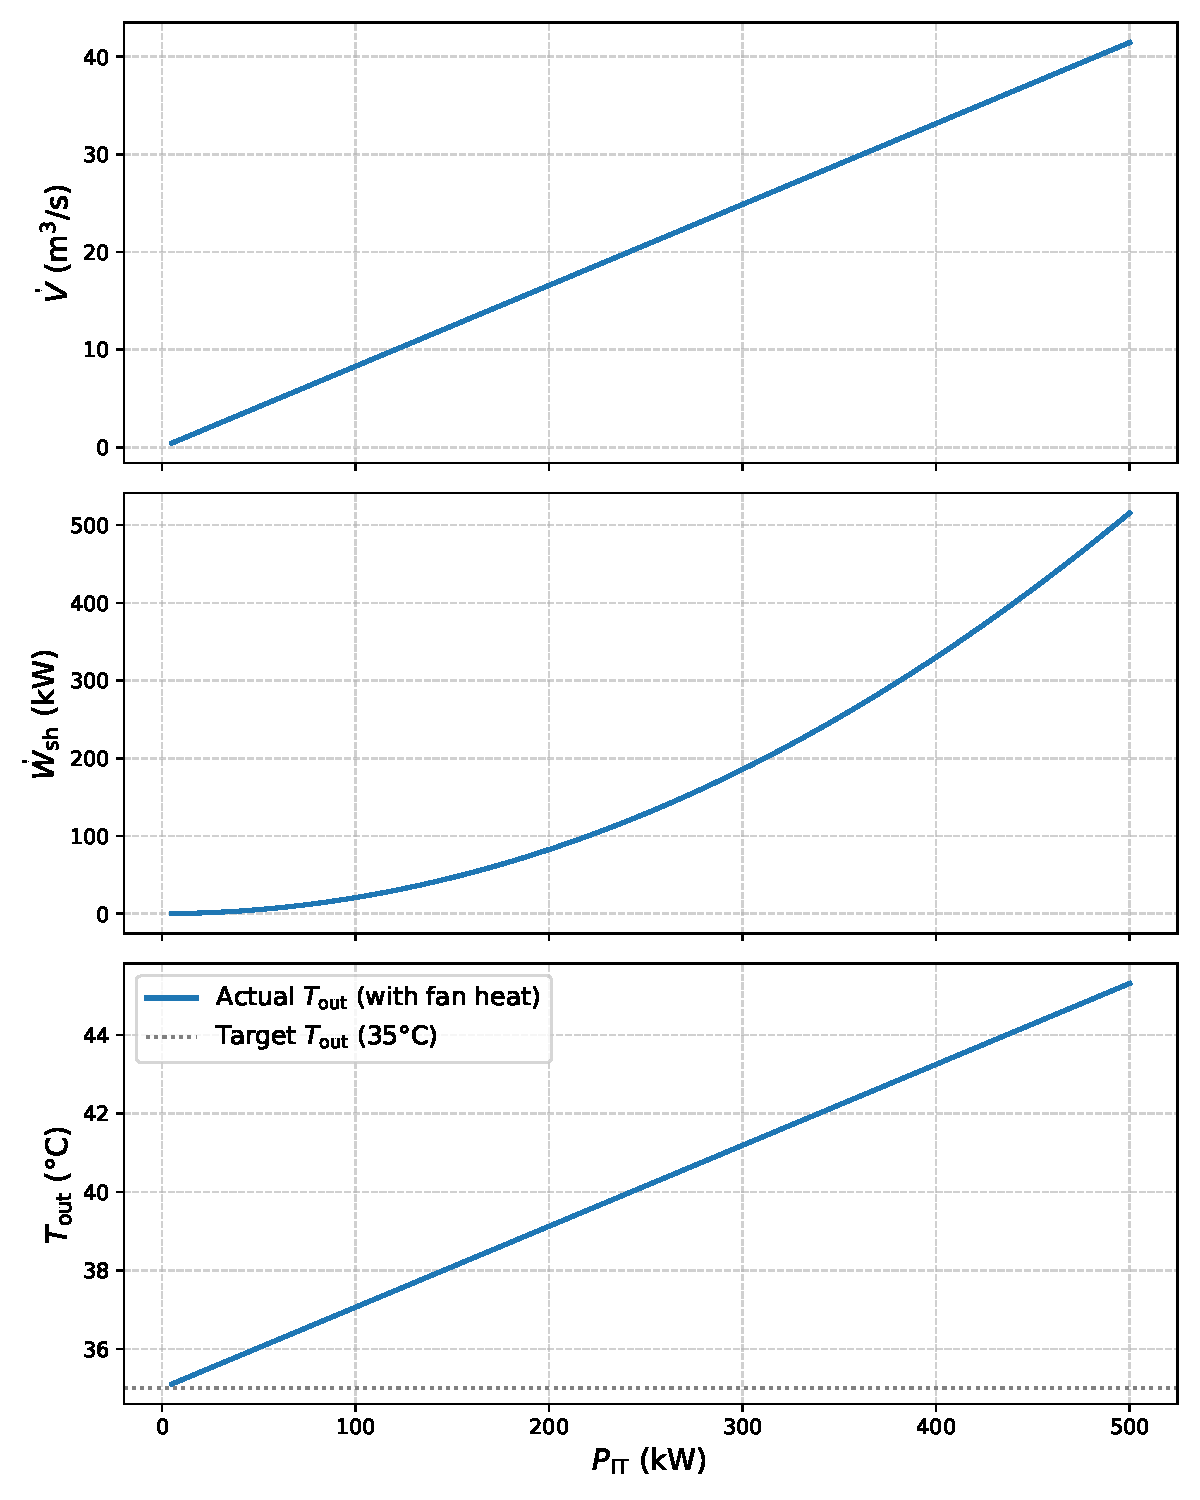
\includegraphics[width=0.4\textwidth]{../figures/rack_cooling_plots.pdf}
%		 \caption{Solution to the Pohlhausen equation. Read his biography \href{https://doi.org/10.1146/annurev.fl.16.010184.000245}{here}.}
%		\end{figure}
%\end{frame}
% ------------------------------------------------------------------------------------------------------------------------------------------------------------------------------------


{
\setbeamertemplate{bibliography item}[text] % Replaces default icons with numbers
	\begin{frame}[allowframebreaks]{References}
		\bibliographystyle{plain}
		\bibliography{../../bibliography}
	\end{frame}
}

}

\end{document}
